
\subsection{Инертные газы и их соединия, способы получения, химическое поведение, электронное и геометрическое строение молекул}

\subsubsection*{Простые вещества}

\textbf{Получение}

1) He, Ar - из природного газа, после сжижения остальных компонентов\\
2) Ne - остаток после сжижения воздуха\\
3) Kr, Xe - селективная адсорбция воздуха углём

\textbf{Химические свойства}

1) Очень низкая химическая активность (вниз по группе растет) (He, Ne, Ar настолько высокие потенциалы ионизации, что истинных хим.соединений не образуют)\\
2) Не поддерживают горения и не возгораются при н.у.\\
3) Реакции Xe:

$$Xe + PtF_6 \rightarrow (Xe^+[PtF_6]^-)$$
По аналогии с реакцией, где вместо $Xe$ был взят $O_2$

Реально получается молекулярный ион $[XeF]^+$\\
В итоге смесь $[XeF]^+[PtF_6]^- + [XeF^+][Pt_2F_{11}]$

С $F_2$

$$Xe + F_2 \xrightarrow{20^{\circ}, UF} XeF_{2(tv)}$$
$$Xe + F_2 \xrightarrow{NiF_2, 100^{\circ}} XeF_6$$
$$Xe + F_2 \xrightarrow{NiF_2, 300^{\circ}}XeF_4$$

C $Au^{3+}$ (как сильный акцептор)

$$AuF_3 + Xe + H^+ \xrightarrow{HF/SbF_5, t^{\circ}} [AuXe_4]^{2+} + [Xe_2]^{2+} + HF$$

$$Au + HF/SbF_5 \xrightarrow{Xe} AuXe_5Sb_2F_{12}$$ 

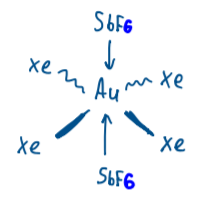
\includegraphics[scale=0.8]{images/13v1.png}

\subsubsection*{Короткоживующие ионы, содержащие Ng}

В газовой фазе встречаются:

$HeH^+, ArH^+$ - молекулярные ионы ( КС=1, но малоустойчивы из-за малой поляризации)\\
Гомоатомные катионы (уменьшение устойчивости вниз по группе)
$He_2^+, Ne_2^+, Ar_2^+, Kr_2^+, Xe_2^+$\\
Очень большая длина связи (> 3 A,  для $Xe_2^+$\\
Существуют, т.к на разрыхляющих орбиталях на 1 электрон меньше, чем на связывающих

\subsubsection*{Клатраты Ng}

Построен по типу "гость-хозяин"\\
Ng "гость" заключенный в решетку "хозяина", не связанный с ним ковалентными связями\\
Получение совместной кристаллизацией при высоком давлении\\
Образование и устойчивость определятся комплементарностью гостя и хозяина (соответствие формы и размера полоски каркаса хозяина размеру сферическому атома Ng )

\textbf{Типы клатратов Ng}

а)  C $H_2O$\\

$24Ng_x136H_2O$ - Ar-Rn\\
$8Ng_x46H_2O$ - Ar-Rn

б)  С гидрохиноном\\

$Ng_x3C_6H_4(OH)_2$ - Ar-Xe

в) C $PhOH$\\

$Ng_x4C_6H_5OH$ - Xe, Rn\\
$Ng_3C_6H_5OH$ -  Ar, Kr\\

г) С пара-$Ph(OH)Cl$\\

$Ng_x3C_6H_4Cl(OH)$ - Xe, Rn

д) с $PHCH_3$

$Ng_x2C_6H_5CH_3$ - Rn

He - настолько маленький, что не способен удерживаться в полостях, клатратов нет

\subsubsection*{Истинные химические соединения}

\textbf{Фториды Xe - наиболее стабильные соединения}

\textbf{Получение}

$$Xe + F_2 \xrightarrow{20^{\circ}, UF} XeF_{2(tv)}$$
$$Xe + F_2 \xrightarrow{NiF_2, 100^{\circ}} XeF_6$$
$$Xe + F_2 \xrightarrow{NiF_2, 300^{\circ}}XeF_4$$

Разделение разгонкой или комплексообразованием

\textbf{Химические свойства}

1) Гидролиз

$$XeF_2 + H_2O \rightarrow Xe + HF + O_2$$
$$XeF_4  + H_2O \rightarrow XeO_3 + Xe + HF + O_2$$
$$XeF_6 + H_2O \rightarrow XeO_3 + HF$$

2) Сильные окислители, фторирующие агенты

$$XeF_2 + S \xrightarrow{HF} SF_6 + Xe$$
$$XeF_2 + Mn(NO_3)_2 + KOH \rightarrow KMnO_4 + KNO_3 + H_2O + Xe + KF$$
$$XeF_2 + CeF_3 \xrightarrow{200^{\circ}} CeF_4 + Xe\uparrow$$
$$XeF_6 + SiO_2 \rightarrow SiF_4 + XeOF_4$$

3) Доноры или (реже) акцепторы $F^-$-анионов

$XeF_2> XeF_6 > XeF_4$\\
$XeF_6 > XeF_4 > XeF_2$

4) С Э$F_5$ (Э = P, Sb, As, Pt) и др. типичными кислотами Льюиса\\
$XeF_2$ дает соли $[XeF]^+[MF_6]^-$ или $[Xe_2F_3]^+[MF_6]$

$$XeF_2 + AsF_5 \rightarrow [XeF]^+[AsF_6]^-$$

Независимо от валентности Xe, образуется часще всего $[XeF]^+$, т.к. E(Xe-F) относительно невелика, и перереход из одного валентного состояния в другое происходит легко

5) Акцепторные свойства ( сфторидами тяжелых ЩМ - Cs или Rb)

$$Cs + XeF_6 \xrightarrow{BrF_5} Cs^+[XeF_7]^-$$
$$Cs^+[XeF_7]^- \xrightarrow{50^{\circ}} Cs_2^+[XeF_8]^{2-} + XeF_6$$

\textbf{Строение}

$XeF_2$ - линейный, $XeF_4$ - квадратный, $XeF_6$ - искаженный октаэдрический (предсказывается по Гиллеспи)

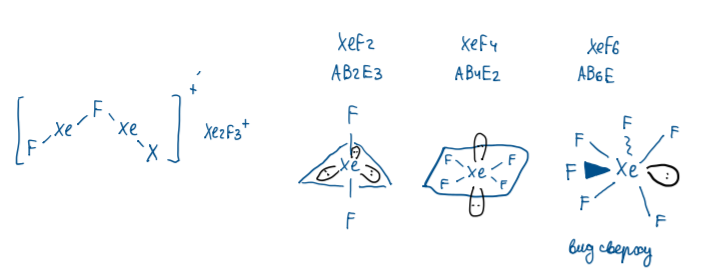
\includegraphics{images/13v2.png}

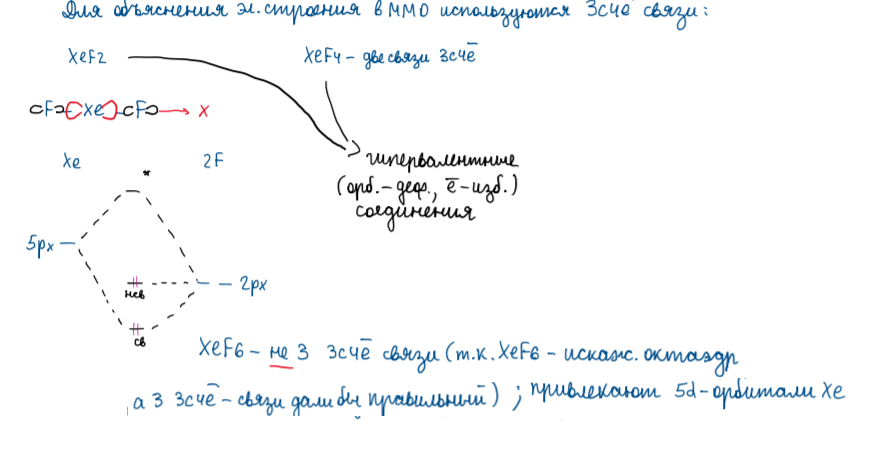
\includegraphics{images/13v3.png}

\textbf{2 оксида $XeO_3$ и $XeO_4$ - оба неустойчивы и легко взрываются}

\textbf{Получение}

$$XeF_6 + H_2O \rightarrow XeO_3 + HF$$
$$XeF_6 + SiO_2 \rightarrow XeO_3 + SIF_4$$
$$Na_4XeO_6 + H_2SO_{4(konc)} Na_2SO_4 + XeO_4 + H_2O$$

\textbf{Химические свойства}

$XeO_3$\\
\\
$$XeO_3 + KOH \rightarrow K[HXeO_4]$$
$$K[HXeO_4] + KOH_{(konc)}  \rightarrow K_4XeO_6 + Xe + O_2 + H_2O$$

$H_2XeO_4$ - ксеноновая кислота, соли ксенаты\\
$H_4XeO_6$ - перксеноновая кислота, соли перксенаны\\

$K_4XeO_6$ - окислитель в реакциях\\
$$K_4XeO_6 + MnO_2 + KOH \rightarrow K_2MnO_4 + Xe + H_2O$$
\\
\\
$XeO_4$\\
\\
$XeO_4$ и $XeO_6^{4-}$ - одни из самых сильных окислителяъ в растворах

В растворах $BrF_5, HF$ - более устойчив

\textbf{Строение}

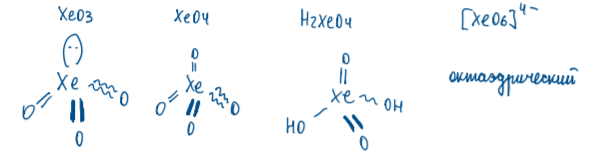
\includegraphics{images/13v4.png}

\textbf{Соединения Rn, Kr}

Соединения Rn не изучены (радиоактивен)\\
Соединения Kr крайней неустойчивы, известен только $KrF_2$ и его производные

\textbf{Получение}

$$KrF_2 \xrightarrow{N_{2(liq)}} KrF_2$$

\textbf{Химические свойтсва}

$$KrF_2 + AsF_5 \rightarrow [KrF]^+[AsF_6]^-$$
$$KrF_2 + SbF_5 \rightarrow [KrF]^+[Sb_6F_{11}]^- + [Kr_2F_3]^+[SbF_6]^-$$

Более сильный окислитель, чем $XeF_2$

$$KrF_2 + MnF_2 \xrightarrow{HF_{liq}} MnF_4 + Kr$$
$$KrF_2 + Au \rightarrow [KrF]^+[AuF_6]^- + Kr$$
$$[KrF]^+[AuF_6]^- \xrightarrow{57^{\circ}} AuF_5 + Kr + F_2$$

C $H_2O$ (бурно, выше $10^{\circ}$)

$$KrF_2 + H_2O \rightarrow Kr + HF + O_2$$ 

Разложение со взрывом на простые вещества при резком нагревании
